\documentclass[tikz,border=3mm]{standalone}
\usepackage[siunitx]{circuitikz}
\usetikzlibrary{calc,positioning,arrows.meta}

\begin{document}

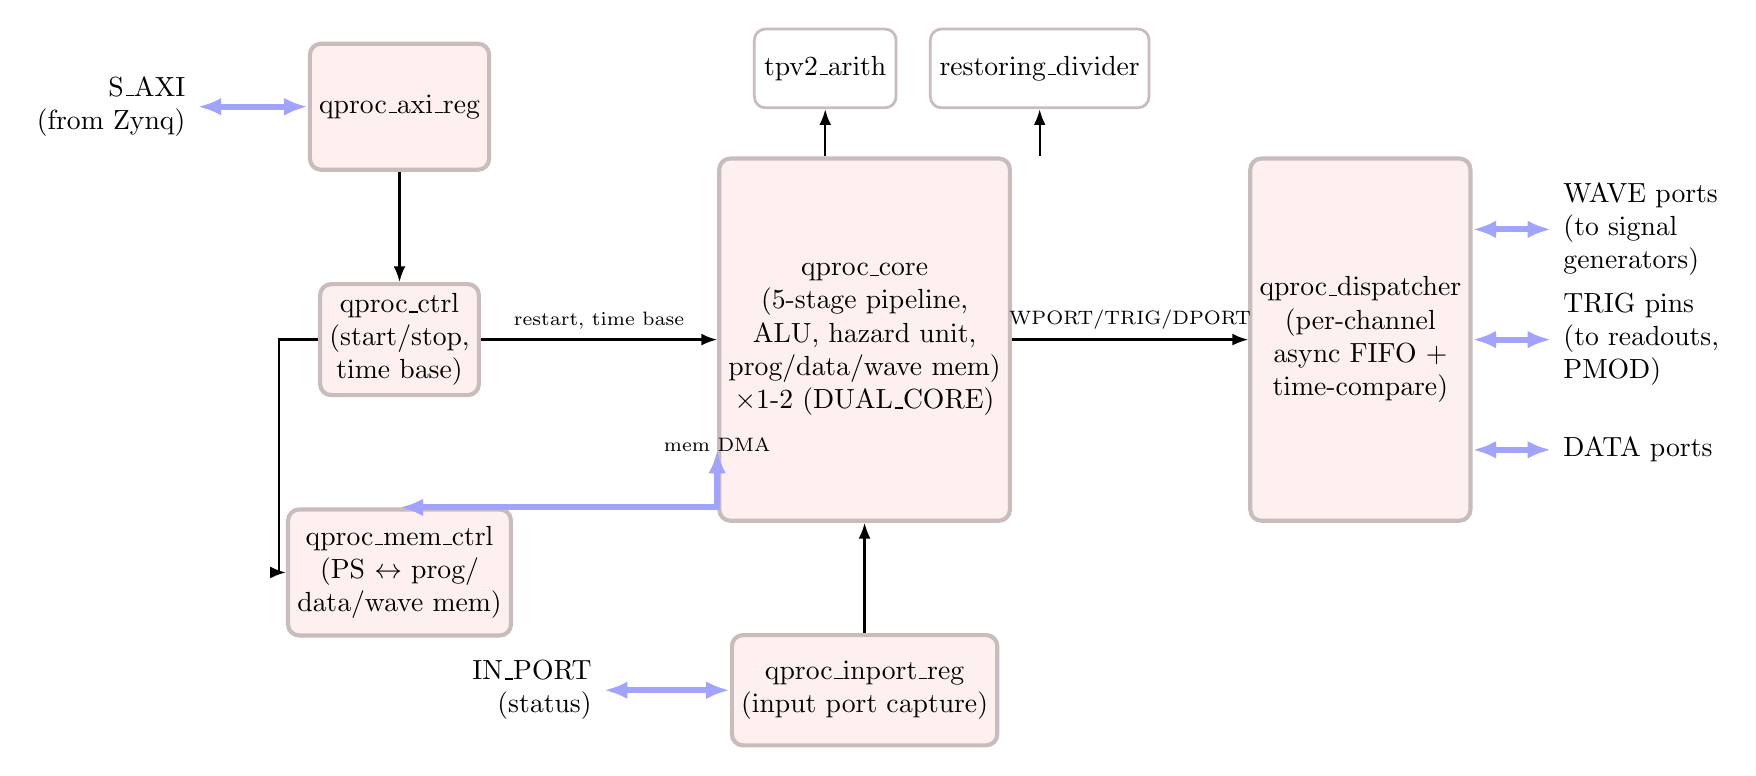
\begin{tikzpicture}
[box/.style={align=center, draw,rounded corners,minimum width=2cm,minimum height=1.2cm,draw={rgb,255:red,200; green,188; blue,188},fill={rgb,255:red,255; green,240; blue,240},line width=1.5pt},
periphbox/.style={align=center, draw,rounded corners,minimum width=1.8cm,minimum height=1cm,draw={rgb,255:red,200; green,188; blue,188},fill=white,line width=1pt},
arrow/.style={line width=2.2pt,draw={rgb,255:red,162; green,163; blue,255},{Latex[length=3mm]}-{Latex[length=3mm]}},
single arrow/.style={line width=0.8pt,-{Latex[length=2mm]}},
node distance=0.6cm]

% Row 1: AXI-Lite register bank.
\node[box,minimum height=1.6cm] (axireg) {qproc\_axi\_reg};

% Row 2: control (left column), core (center), dispatcher (right).
\node[box,below=1.4cm of axireg,minimum height=1.4cm] (ctrl) {qproc\_ctrl\\(start/stop,\\ time base)};

\node[box,right=3cm of ctrl,minimum height=4.6cm,minimum width=3cm] (core) {qproc\_core\\(5-stage pipeline,\\ ALU, hazard unit,\\ prog/data/wave mem)\\ $\times$1-2 (DUAL\_CORE)};

\node[box,right=3cm of core,minimum height=4.6cm,minimum width=2.6cm] (disp) {qproc\_dispatcher\\(per-channel\\ async FIFO +\\ time-compare)};

% Peripherals, stacked to the right of the core's top, left of dispatcher.
\node[periphbox,above=0.6cm of core,xshift=-0.5cm] (arith) {tpv2\_arith};
\node[periphbox,right=0.4cm of arith] (div) {restoring\_divider};

% Row 3: PS memory DMA (below ctrl), input port capture (below core).
\node[box,below=1.4cm of ctrl,minimum height=1.6cm] (memctrl) {qproc\_mem\_ctrl\\(PS $\leftrightarrow$ prog/\\data/wave mem)};

\node[box,below=1.4cm of core,minimum height=1.4cm,minimum width=3cm] (inport) {qproc\_inport\_reg\\(input port capture)};

% s_axi.
\draw[arrow] ($(axireg.west)+(-1.4,0)$) node[anchor=east,align=right] {S\_AXI\\(from Zynq)} -- (axireg.west);

% axireg -> ctrl (start/stop, time regs).
\draw[single arrow] (axireg.south) -- (ctrl.north);

% axireg -> memctrl (PS bulk access to memories).
\draw[single arrow] (ctrl.west) -- ++(-0.5,0) |- (memctrl.west);

% ctrl -> core (restart/time base).
\draw[single arrow] (ctrl.east) -- (core.west) node[pos=0.5,above,font=\scriptsize] {restart, time base};

% memctrl <-> core (PS DMA into prog/data/wave mem): up from memctrl, then
% right into core's bottom-left.
\coordinate (memctrl up) at (memctrl.north -| core.west);
\draw[arrow] (memctrl.north) -- (memctrl up) -- ($(core.west)+(0,-1.4)$) node[pos=0.75,above,font=\scriptsize,align=center] {mem DMA};

% core <-> peripherals.
\draw[single arrow] (core.north -| arith) -- (arith.south);
\draw[single arrow] (core.north -| div) -- (div.south);

% inport -> core.
\draw[single arrow] (inport.north) -- (core.south -| inport.north);

% Input ports (from generators/readouts, trigger/ack/status).
\draw[arrow] ($(inport.west)+(-1.6,0)$) node[anchor=east,align=right] {IN\_PORT\\(status)} -- (inport.west);

% core -> dispatcher (WPORT_WR/TRIG/DPORT_WR).
\draw[single arrow] (core.east) -- (disp.west) node[pos=0.5,above,font=\scriptsize] {WPORT/TRIG/DPORT};

% dispatcher outputs.
\coordinate (wave out) at ($(disp.east)+(0,1.4)$);
\coordinate (trig out) at ($(disp.east)+(0,0)$);
\coordinate (dport out) at ($(disp.east)+(0,-1.4)$);
\draw[arrow] (wave out) -- ++(1,0) node[anchor=west,align=left] {WAVE ports\\(to signal\\ generators)};
\draw[arrow] (trig out) -- ++(1,0) node[anchor=west,align=left] {TRIG pins\\(to readouts,\\ PMOD)};
\draw[arrow] (dport out) -- ++(1,0) node[anchor=west,align=left] {DATA ports};

\end{tikzpicture}

\end{document}
